This section will characterize the Drupal service, providing the rationale for the system design that follows in section \ref{sec-k8s-design}.

The service supports website admins to host and administer websites directed to the grand public,
such as experiment or departmental central websites.
Some of the most popular sites based on this service are \href{https://home.cern/}{home.cern}, \href{https://atlas.cern}{atlas.cern},
\href{https://cms.cern}{cms.cern}, \href{https://careers.cern}{careers.cern} and \href{https://visit.cern}{visit.cern}.
As such they form CERN's main outreach channel and are critical for the Organization's reputation.

Users of the service range across a wide spectrum of different professional profiles,
and it's quite common that the responsibility of site building at CERN falls on administrative personnel, or personnel with little technical background in web technologies.
This in turn shapes the kind of service we have to provide; contrary to developer communities best practices, it is, for example, impractical to rely exclusively on developer-centric workflows, like GitOps and CLI tools.
A small fraction of our user base, however, indeed have web development experience.

% TODO Pick smt from White Area talk.

The consequence is that the Drupal service has a dual mission:
\begin{enumerate}
    \item to ensure the \emph{high availability} and performance of these communication channels
    \item to make site building and administration accessible to a user base with wide-ranging technical background, while remaining extensible for websites needing special features
\end{enumerate}

This work describes an infrastructure project that focuses on furthering the \emph{first mission}, without sacrificing the second.
Ideally, the changes should be almost transparent for non-technical site administrators, while enabling previously unavailable best-practices workflows for technical users.

\subsubsection*{Portfolio of web frameworks}

In order to provide flexible solutions to the needs of the Organization's diverse community, CERN IT supports a portfolio of web hosting and content creation platforms based on different technologies, collectively called Web Frameworks.
In table \ref{tab-wf} are some Web Frameworks and indicative use cases.

\begin{table}[h!]
\begin{tabularx}{\textwidth}{ p{10em}| >{\raggedright\arraybackslash}X}
\emph{Name} & \emph{Indicative use case} \\
\hline \\
Apache web hosting & Serve static HTML/CSS/JS/CGI stored on the EOS shared filesystem with simple deployment requirements \\
CMS/Drupal & \hyperref[what-is-drupal]{Content Management System} for visual content creation and public outreach \\
Platform as a Service (PaaS) & Custom web applications with flexible deployment on Openshift (Kubernetes) \\
Discourse & A home for communities around a common topic \\
TWiki & Wiki format content creation platform
\end{tabularx}
\caption{Some Web Frameworks at CERN}
\label{tab-wf}
\end{table}

For each web framework there is currently a separate infrastructure, developed with different and not interoperable technologies.
This creates silos of operational expertise within the small engineering team that supports each one, which are costly and inefficient to keep alive in CERN's dynamic working environment.
At the same time there are a lot of software components developed in-house to support a single use case at the time, generating a large technical debt.
Many requirements however are common, such as interfacing with external CERN systems.

There is an obvious benefit in consolidating the web frameworks on a common infrastructure.
In the context of this project, such a common Kubernetes-based infrastructure is being developed,
with many shared components and only a thin business logic layer specific to each use case.

\subsection{Technical characteristics of the service}

\subsubsection*{Website customization}

All websites on the infrastructure are running the same Drupal distribution in a "multi-site" configuration, as will be explained in section \ref{sec-phys-infra}.
The distribution consists of an upstream Drupal version with a few patches for the CERN environment, plus a curated set of "central" modules.
This puts control of the code, and critically, \emph{security updates}, in the hands of the infrastructure team.
However, many websites need extra features and Drupal was selected exactly \hyperref[drupal-at-cern]{because of its extensibility}.
It is possible for website admins to upload community modules, thereby extending Drupal specifically for their website.

\subsubsection*{Development workflow}

Two types of website are supported administratively, corresponding to different Quality of Service (QoS) expectations: official (production) and test (test and development).
There is currently no concept of \emph{"environments"} or branches. Developing a website involves maintaining a production website and one or more independent development websites.
Data can be cloned between websites, so that the development website reproduce the production one.

A site admin that wants to safely develop a new content type or view, add a new module, or even change configuration, should start by cloning the production website to a development website.
They need to keep track of changes, then reproduce them on the production website.
There is no GitOps.

Despite seeming inefficient from a software engineering perspective, this workflow is acceptable by most website admins.
The ones with development experience though would benefit significantly from version controlling configuration changes and extra modules.
A Git-based workflow will be enabled with this work.

\subsection{Load characteristics}

\href{https://home.cern/}{home.cern} is the most public website at CERN.
Out of 1043 Drupal websites currently hosted, it alone serves 32\% of monthly unique visitors.
The top 10 websites together serve 79\% of all unique visitors, leaving only 1/5 among them headed for the other 1033 websites.
This is an intrinsic characteristic of the service load, which is heavily skewed towards a very small number of critical websites.

Unique visitors is a good measure of a website's publicity, but a measure that is easier to assess an infrastructure on is the number of HTTP requests.
The situation there is similar, with the top 10 websites being the target of 60\% of all requests.
In section \ref{sec-experiment} we will describe an experiment on resource optimization by assigning websites to different Quality of Service classes,
according to their needs, where both metrics are relevant.


\subsubsection*{Concurrent requests}

\begin{wrapfigure}{r}{.46\textwidth}
\centering
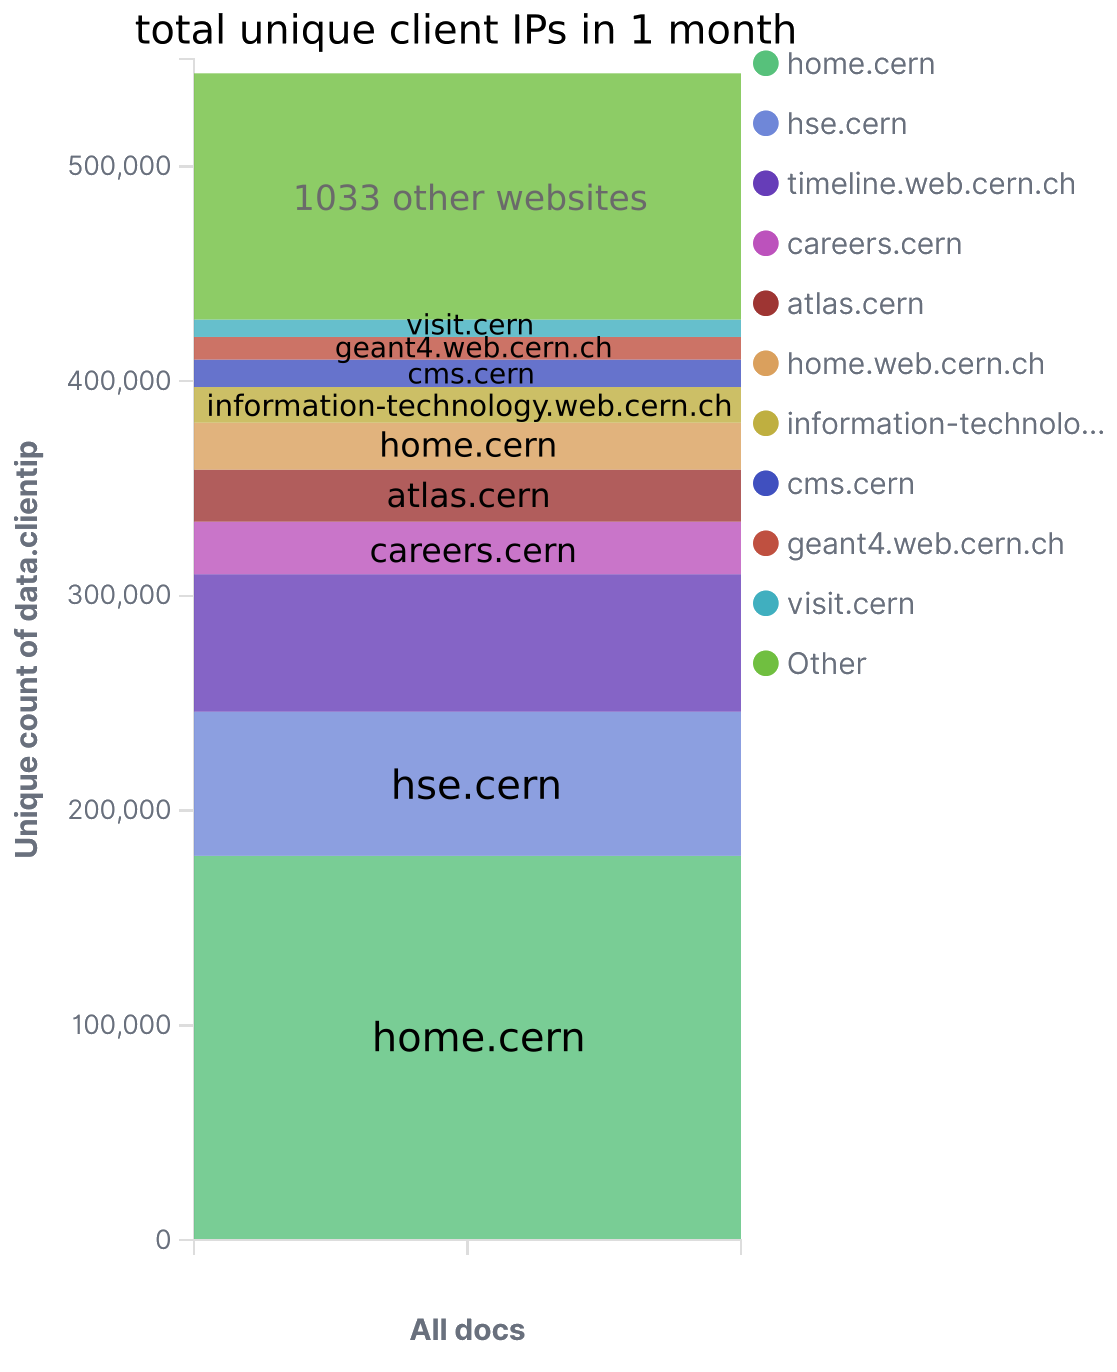
\includegraphics[width=.50\textwidth]{figures/drupal-top10-uniqClientIP.png}
\caption{Calculating the unique client IPs over a month from Apache logs and grouping per site
is taken as a proxy measure of a site's publicity, or how much impact it has on the Organization's reputation.
In this figure the top 10 most public Drupal websites are shown.
home.cern appears twice as home.cern and home.web.cern.ch (but it's the same website)
}
\label{fig-drp-top10-cip}
\end{wrapfigure}

% TODO
\begin{figure}
    \centering
    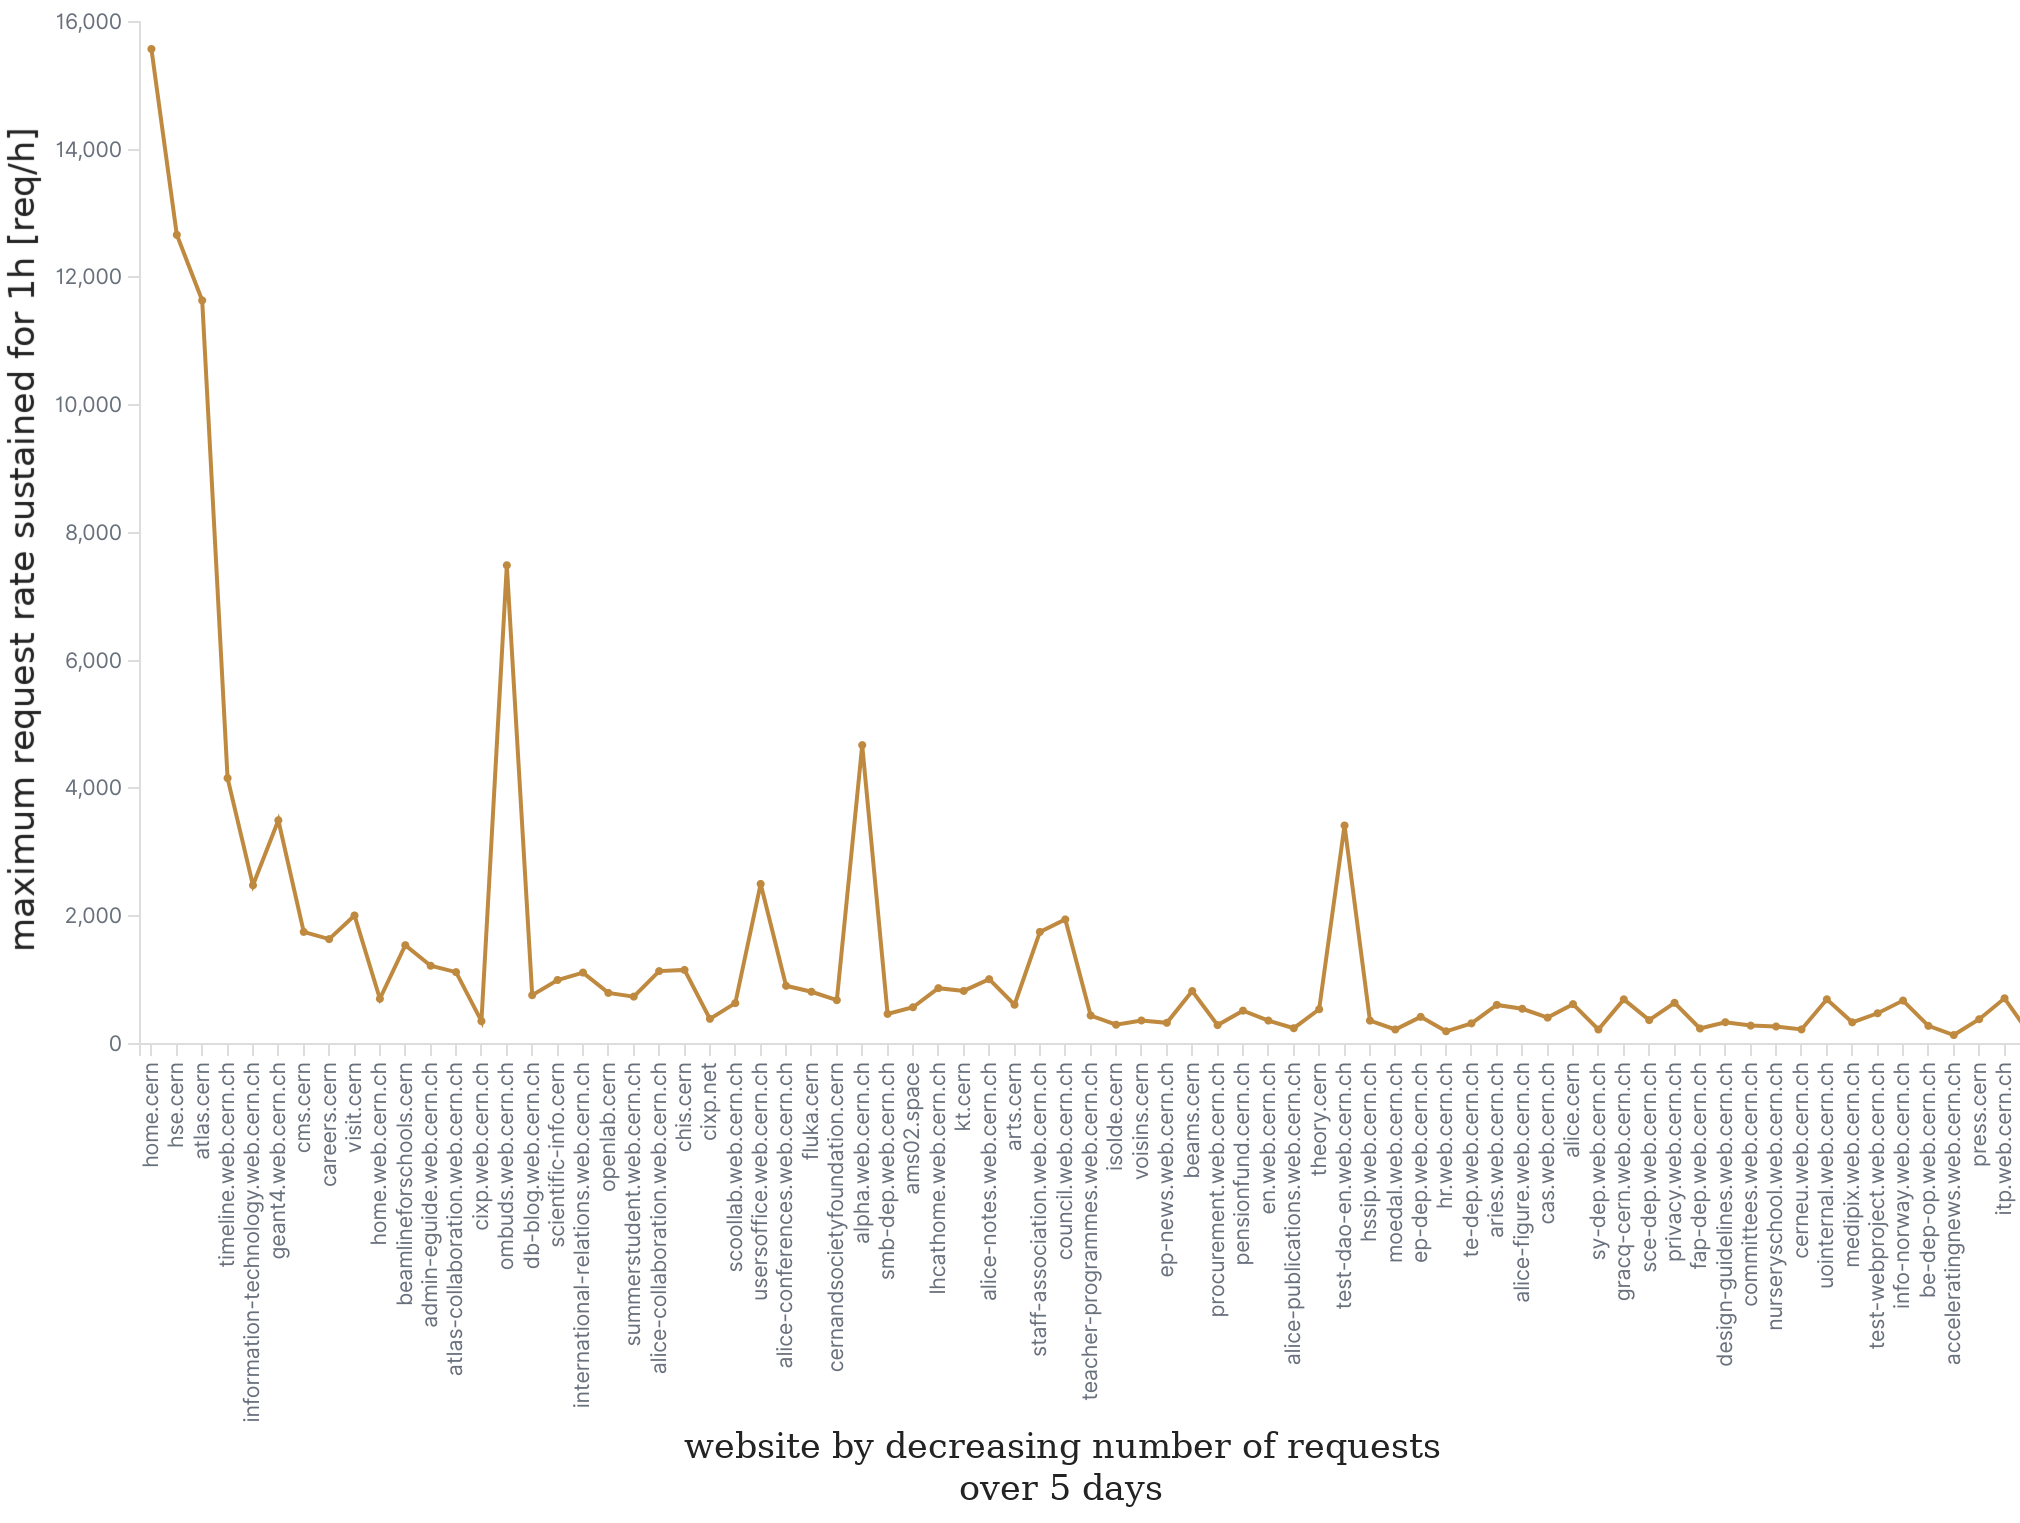
\includegraphics[width=1.05\textwidth]{figures/website-bandwidth}
    \caption{\emph{Website maximum bandwidth}.
      The websites on the infrastructure have rather low bandwidth}
    \label{fig:my_label}
\end{figure}

%TODO Change from here on end users to Requests per second and anything related 
How many end users access a single site simultaneously?
How many should the website be able to handle without slowing down?
To better understand how the load impacts a single website (and therefore estimate the required hosting resources),
we performed some measurements.
We searched in historical data for periods where the load peaks on the infrastructure
and noted the maximum number of unique client IPs accessing the same website over a period of 10 minutes:
226 concurrent clients connected to home.cern

The loading time of pages at home.cern without load is slightly over 1 second, which is acceptable.
Let a legitimate client request pages from home.cern as soon as the previous page has been delivered (similar to a web crawler).
This would result in an upper bound request rate of $600 \times 226 = 135k$ requests per 10 minutes.
The actual request rate observed across the entire infrastructure when load peaks is much lower, 46k.

These observations align with expectations and requirements: critical websites should be able to handle 200 simultaneous legitimate clients without slowdown.

% NOTES
=> define num of users for QoS classes
% NOTES


%%%%
% NOTES
%%%%

% <graph: kibana top10 uniqueIP stacked bar> https://monit-timber-drupal-prod8.cern.ch/kibana/app/kibana#/visualize/create?type=histogram&indexPattern=d2ef41c0-e515-11e9-886e-69c303354aa9&_g=(refreshInterval:(pause:!t,value:0),time:(from:now-1M,to:now))&_a=(filters:!(),linked:!f,query:(language:kuery,query:'data.program:%22httpd%22'),uiState:(),vis:(aggs:!((enabled:!t,id:'1',params:(field:data.clientip),schema:metric,type:cardinality),(enabled:!t,id:'2',params:(field:data.sitename,missingBucket:!f,missingBucketLabel:Missing,order:desc,orderBy:'1',otherBucket:!t,otherBucketLabel:Other,size:10),schema:group,type:terms)),params:(addLegend:!t,addTimeMarker:!f,addTooltip:!t,categoryAxes:!((id:CategoryAxis-1,labels:(show:!t,truncate:100),position:bottom,scale:(type:linear),show:!t,style:(),title:(),type:category)),grid:(categoryLines:!f),legendPosition:right,seriesParams:!((data:(id:'1',label:'Unique%20count%20of%20data.clientip'),drawLinesBetweenPoints:!t,mode:stacked,show:true,showCircles:!t,type:histogram,valueAxis:ValueAxis-1)),times:!(),type:histogram,valueAxes:!((id:ValueAxis-1,labels:(filter:!f,rotate:0,show:!t,truncate:100),name:LeftAxis-1,position:left,scale:(mode:percentage,type:linear),show:!t,style:(),title:(text:'Unique%20count%20of%20data.clientip'),type:value))),title:'New%20Visualization',type:histogram))

% <graph: kibana top10 requests stacked bar>  https://monit-timber-drupal-prod8.cern.ch/kibana/app/kibana#/visualize/create?type=histogram&indexPattern=d2ef41c0-e515-11e9-886e-69c303354aa9&_g=(filters:!(),refreshInterval:(pause:!t,value:0),time:(from:now-1M,to:now))&_a=(filters:!(('$state':(store:appState),meta:(alias:!n,disabled:!f,index:d2ef41c0-e515-11e9-886e-69c303354aa9,key:data.sitename,negate:!t,params:(query:test-jardin-de-particules-d8.web.cern.ch),type:phrase,value:test-jardin-de-particules-d8.web.cern.ch),query:(match:(data.sitename:(query:test-jardin-de-particules-d8.web.cern.ch,type:phrase)))),('$state':(store:appState),meta:(alias:!n,disabled:!f,index:d2ef41c0-e515-11e9-886e-69c303354aa9,key:data.sitename,negate:!t,params:(query:test-uo-bat.web.cern.ch),type:phrase,value:test-uo-bat.web.cern.ch),query:(match:(data.sitename:(query:test-uo-bat.web.cern.ch,type:phrase)))),('$state':(store:appState),meta:(alias:!n,disabled:!f,index:d2ef41c0-e515-11e9-886e-69c303354aa9,key:data.sitename,negate:!t,params:(query:test-lpcc.web.cern.ch),type:phrase,value:test-lpcc.web.cern.ch),query:(match:(data.sitename:(query:test-lpcc.web.cern.ch,type:phrase)))),('$state':(store:appState),meta:(alias:!n,disabled:!f,index:d2ef41c0-e515-11e9-886e-69c303354aa9,key:data.sitename,negate:!t,params:(query:test-missionlhc.web.cern.ch),type:phrase,value:test-missionlhc.web.cern.ch),query:(match:(data.sitename:(query:test-missionlhc.web.cern.ch,type:phrase))))),linked:!f,query:(language:kuery,query:'data.program:%22httpd%22'),uiState:(),vis:(aggs:!((enabled:!t,id:'1',params:(),schema:metric,type:count),(enabled:!t,id:'2',params:(field:data.sitename,missingBucket:!f,missingBucketLabel:Missing,order:desc,orderBy:'1',otherBucket:!t,otherBucketLabel:Other,size:10),schema:group,type:terms)),params:(addLegend:!t,addTimeMarker:!f,addTooltip:!t,categoryAxes:!((id:CategoryAxis-1,labels:(show:!t,truncate:100),position:bottom,scale:(type:linear),show:!t,style:(),title:(),type:category)),grid:(categoryLines:!f),legendPosition:right,seriesParams:!((data:(id:'1',label:Count),drawLinesBetweenPoints:!t,mode:stacked,show:true,showCircles:!t,type:histogram,valueAxis:ValueAxis-1)),times:!(),type:histogram,valueAxes:!((id:ValueAxis-1,labels:(filter:!f,rotate:0,show:!t,truncate:100),name:LeftAxis-1,position:left,scale:(mode:percentage,type:linear),show:!t,style:(),title:(text:Count),type:value))),title:'New%20Visualization',type:histogram))